
\chapter{Zodiacal Light}

\lettrine[lines = 4]{\goudy I}{n} order to complete our view of all that we have learned to consider as appertaining to our solar system, which now, since the discovery of the small planets, of the interior comets of short revolutions, and of the meteoric asteroids, is so rich and complicated in its form, it remains for us to speak of the ring of zodiacal light, to which we have already alluded. Those who have lived for many years in the zone of palms must retain a pleasing impression of the mild radiance with which the zodiacal light, shooting pyramidally upward, illumines a part of the uniform length of tropical nights. I have seen it shine with an intensity of light equal to the Milky Way in Sagittarius, and that not only in the rare and dry atmosphere of the summits of the Andes, at an elevation of from thirteen to fifteen thousand feet, but even on the boundless grassy plains, the llanos of Venezuela, and on the seashore, beneath the ever-clear sky of Cumana. This phenomenon was often rendered especially beautiful by the passage of light, fleecy clouds, which stood out in picturesque and bold relief from the luminous background. A notice of this aerial spectacle is contained in a passage in my journal, while I was on the voyage from Lima to the western coasts of Mexico. For three or four nights (between 10 and 14 north latitude) the zodiacal light has appeared in greater splendor than I have ever observed it. The transparency of the atmosphere must be remarkably great in this part of the Southern Ocean, to judge by the radiance of the stars and nebulous spots. From the 14th to the 19th of March a regular interval of three quarters of an hour occurred between the disappearance of the sun's disk in the ocean and the first manifestation of the zodiacal light, although the night was already perfectly dark. An hour after sunset it was seen in great brilliancy between Aldebaran and the Pleiades; and on the 18th of March it attained an altitude of 39 5. Narrow elongated clouds are scattered over the beautiful deep azure of the distant horizon, flitting past the zodiacal light as before a golden curtain. Above these, other clouds are from time to time reflecting the most brightly variegated colors. It seems a second sunset. On this side of the vault of heaven the lightness of the night appears to increase almost as much as at the first quarter of the moon. Toward 10 o'clock the zodiacal light generally becomes very faint in this part of the Southern Ocean, and at midnight have scarcely been able to trace a vestige of it. On the 16th of March, when most strongly luminous, a faint reflection was visible in the east. In our gloomy so-called "temperate" northern zone, the zodiacal light is only distinctly visible in the beginning of Spring, after the evening twilight, in the western part of the sky, and at the close of Autumn, before the dawn of day, above the eastern horizon.

%\clearpage
\begin{wrapfigure}{r}{0.4\textwidth}
   \vspace{-30pt}
   \begin{center}
      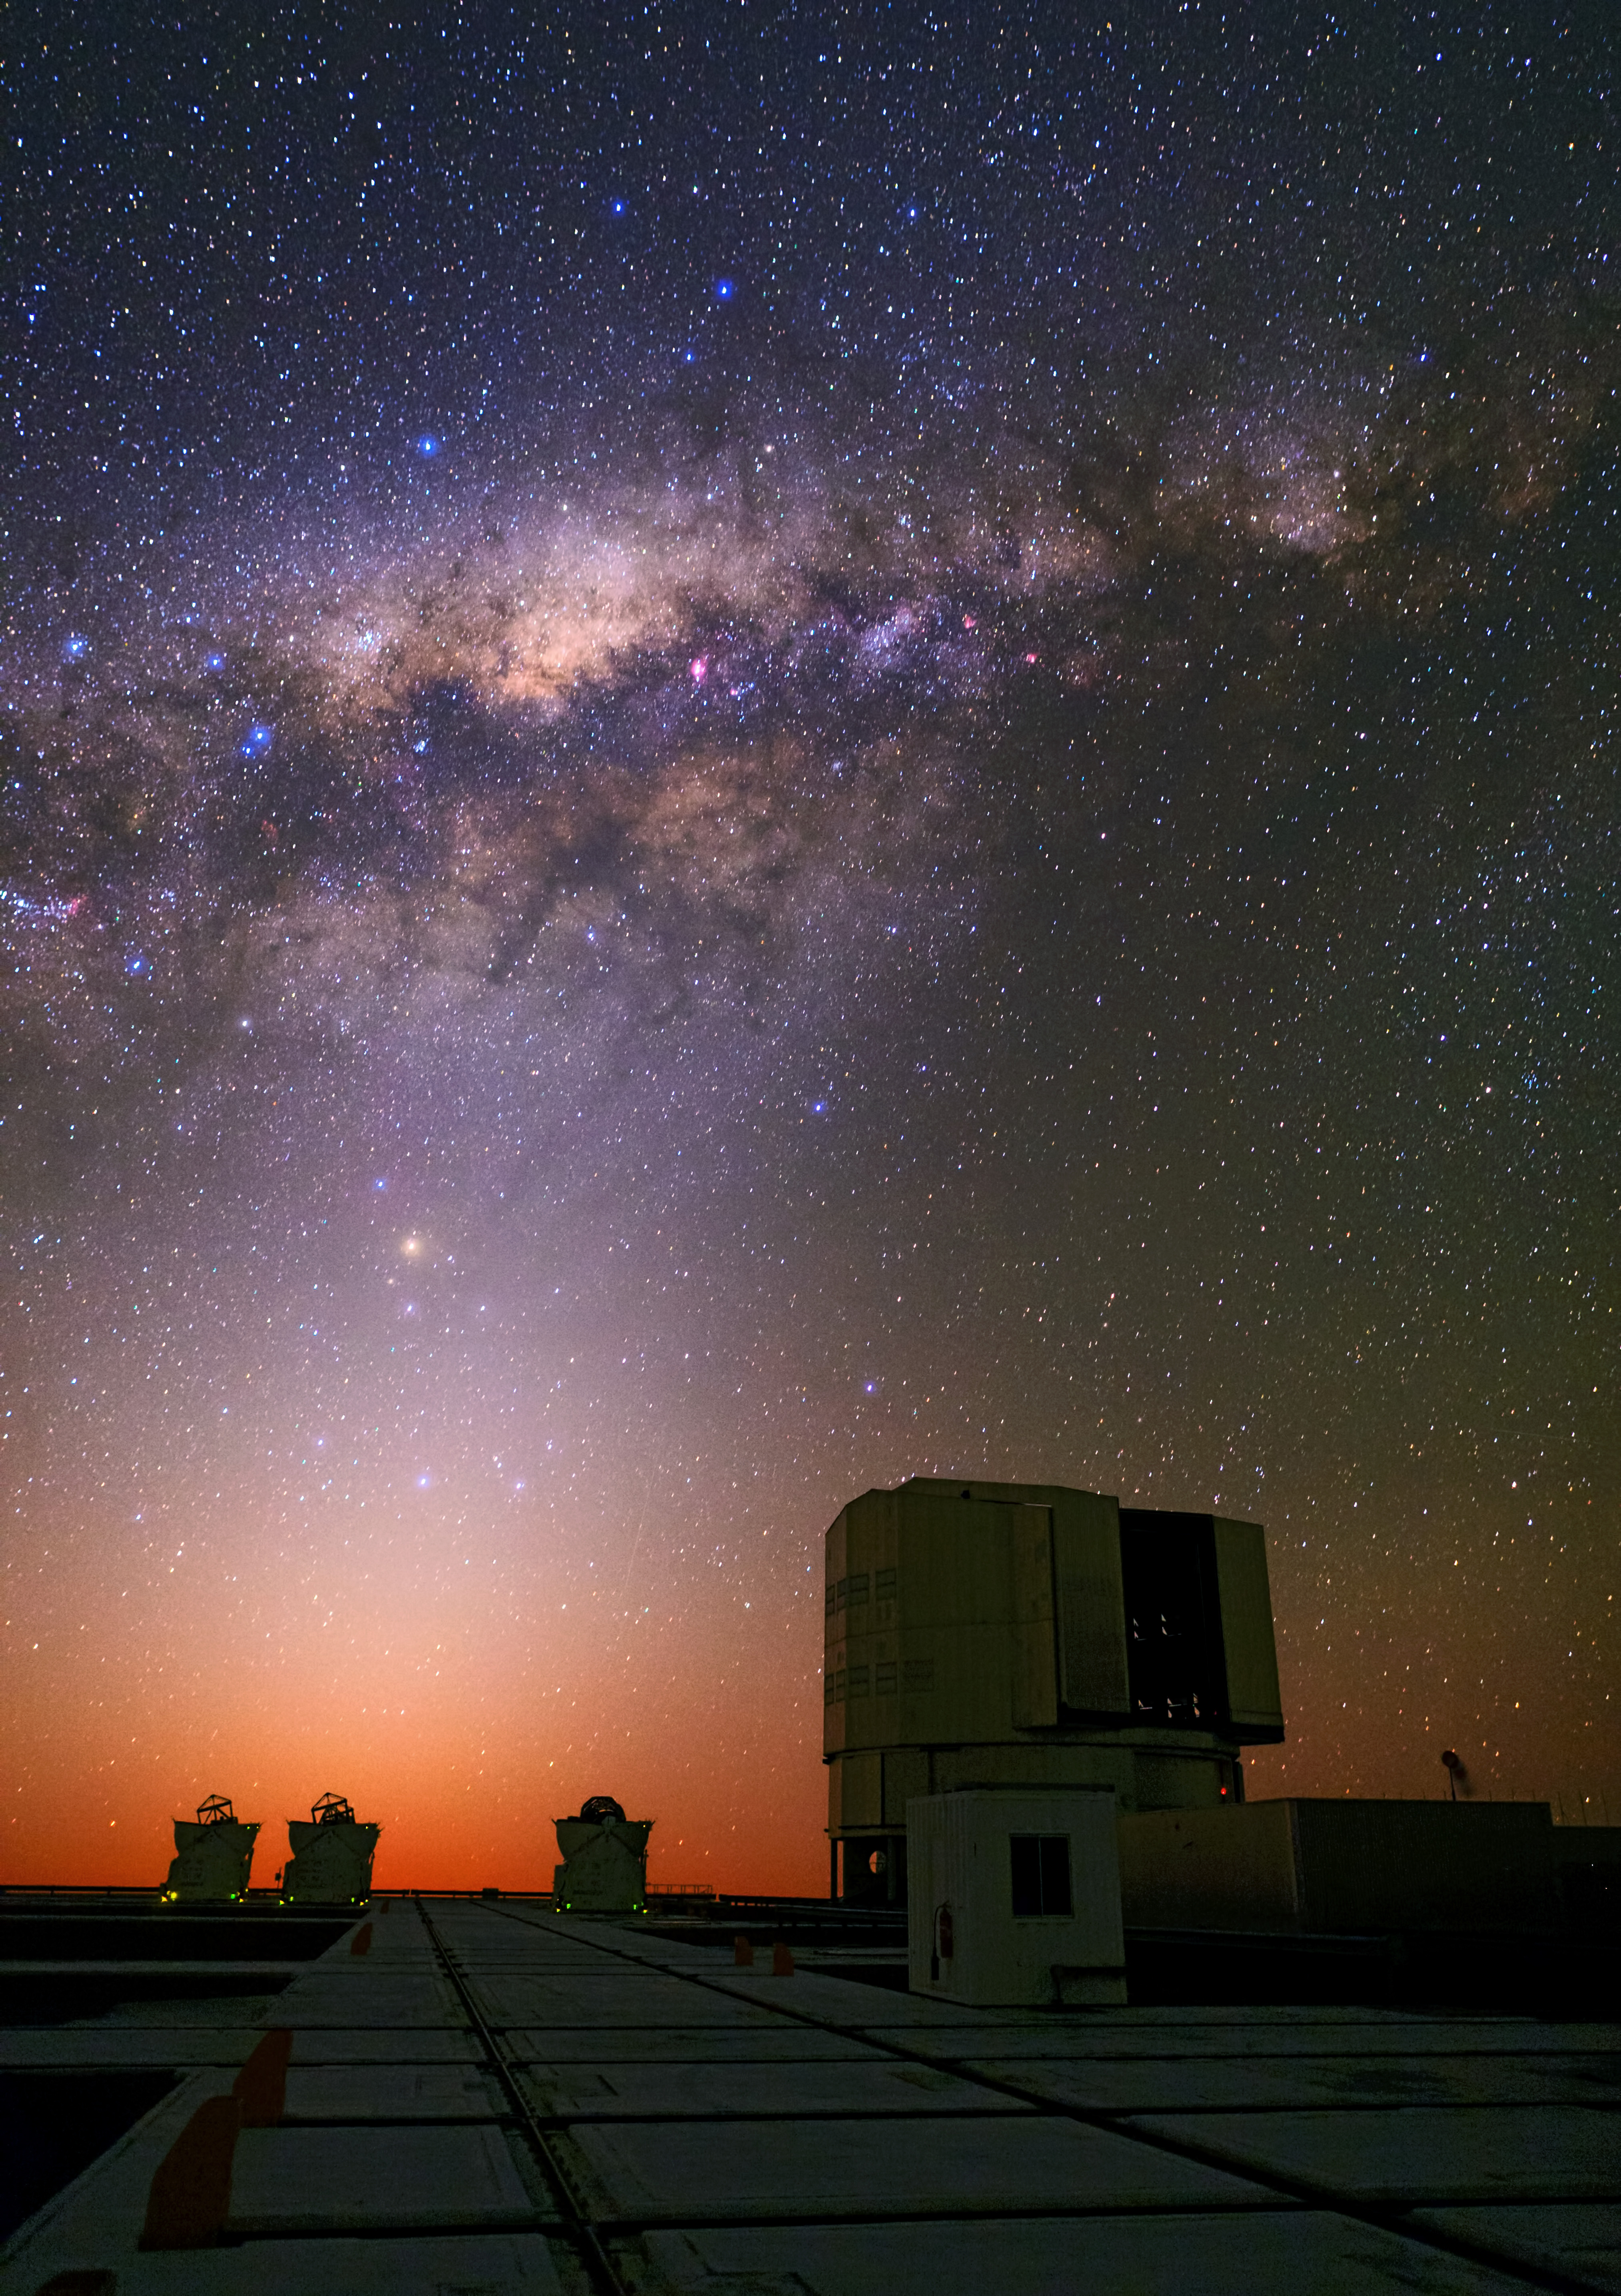
\includegraphics[width=0.4\textwidth]{../../pictures/Romantic_Sunset_over_the_VLT.jpg}
   \end{center}
   \vspace{-15pt}
   \caption{
      {\footnotesize Centre of the Milky Way and zodiacal light above the platform of the Very Large
            Telescope (VLT) on Cerro Paranal. Author:
            \href{https://commons.wikimedia.org/wiki/File:Romantic_Sunset_over_the_VLT.jpg}{ESO/B. Tafreshi
               (twanight.org)}. License: \href{https://creativecommons.org/licenses/by/4.0/deed.en}{CC BY 4.0}.}
   }
   \label{fig:zodiacal_light}
   %\end{adjustbox}
\end{wrapfigure}
It is difficult to understand how such a striking natural phenomenon could have failed to attract the attention of physicists and astronomers until the middle of the seventeenth century, or how it could have escaped the observation of the Arabian natural philosophers in ancient Bactria, on the Euphrates, and in the south of Spain. Almost equally surprising is the tardiness of observation of the nebulous spots in Andromeda and Orion, first described by Simon Marius and Huygens. The earliest explicit description of the zodiacal light occurs in Childrey's Britannia Baconica\footnote{There is another thing which I recommend to the observation of mathematical men, which is, that in February, and for a little before and a little after that month (as I have observed several years together), about six in the evening, when the twilight has almost deserted the horizon, you shall see a plainly discernible way of the twilight striking up toward the Pleiades, and seeming almost to touch them. It is so observed any clear night, but it is best illac nocte. There is no such way to be observed at any other time of the year (that I can perceive), nor any other way at that time to be perceived darting up elsewhere; and I believe it has been, and will be constantly visible at that time of the year; but what the cause of it in nature should be, I cannot yet imagine, but leave it to future inquiry. (Childrey, Britannia Baconica, 1661, p. 183.) This is the first view and a simple description of the phenomenon. (Cassini, Découverte de la Lumière Céleste qui parott dans le Zodiaque, in the Mém. de l'Acad., t. viii., 1730, p. 276. Mairan, Traité Phys. de l'Aurore Boréale, 1754, p.16.) In this remarkable work by Childrey, there are very clear accounts of the epochs of maximum and minimum diurnal and annual temperatures, and of the retardation of the extremes of the effects in meteorological processes. It is, however, to be regretted that our Baconian philosophy-loving author, who was Lord Henry Somerset's chaplain, fell into the same error as Bernardin de St. Pierre and regarded the Earth as elongated at the poles (see p. 148). At first, he believes that the Earth was spherical but supposes that the uninterrupted and increasing addition of layers of ice at both poles has changed its figure; and that, as the ice is formed from water, the quantity of that liquid is everywhere diminishing.}, in the year 661. The first observation of the phenomenon may have been made two or three years prior to this period; but, notwithstanding, the merit of having (in the spring of 1683) been the first to investigate the phenomenon in all its relations in space is incontestably due to Dominicus Cassini. The light which he saw at Bologna in 1668, and which was observed at the same time in Persia by the celebrated traveler Chardin (the court astrologers of Ispahan called this light, which had never before been observed, nyzek, a small lance), was not the zodiacal light, as has often been asserted,\footnote{Dominicus Cassini (Mém. de l'Acad., t. viii, 1730, p. 188), and Mairan (Aurore Bor., p. 16), have even maintained that the phenomenon observed in Persia in 1668 was the zodiacal light. Delambre (Hist. de Astron. Moderne, t. ii., p. 742), in very decided terms, ascribes the discovery of this light to the celebrated traveler Chardin; but in the Couronnement de Soliman, and in several passages of the narrative of his travels (éd. de Langlès, t. iv., p. 326; t. x., p. 97), he only applies the term niazouk (nyzek), or petite lance, to the great and famous comet which appeared over nearly the whole world in 1668, and whose head was so hidden in the west that it could not be perceived on the horizon of Ispahan (Atlas du Voyage de Chardin, Tap. iv.; from the observations at Schiraz). The head or nucleus of the comet was, however, visible in the Brazils and in India (Pingré, Cométogr., t. ii., p. 22). Regarding the conjectured identity of the last great comet of March 1843 with this, which Cassini mistook for the zodiacal light, see Schum., Astr. Nachr., 1843, No. 476 and 480. In Persian, the term nizehiteschin (fiery spears or lances) is also applied to the rays of the rising or setting sun, in the same way as nayazik, according to Freytag's Arabic Lexicon, signifies "stelle cadentes." The comparison of comets to lances and swords was, however, very common in all languages in the Middle Ages. The great comet of 1500, which was visible from April to June, was always termed by the Italian writers of that time "el Signor Astone" (see my Examen Critique de l'Hist. de la Géographie, t. v., p. 80). All the hypotheses that have been advanced to show that Descartes (Cassini, p. 230; Mairan, p. 16), and even Kepler (Delambre, t. i., p. 601), were acquainted with the zodiacal light, appear to me altogether untenable. Descartes (Principes, iii., art. 136, 137) is very obscure in his remarks on comets, observing that their tails are formed by oblique rays, which, falling on different parts of the planetary orbs, strike the eye laterally by extraordinary refraction, and that they might be seen morning and evening, like a long beam, when the Sun is between the comet and the Earth. This passage no more refers to the zodiacal light than those in which Kepler (Eyit. Astron. Copernicana, t.i., p. 57, and t. ii., p. 893) speaks of the existence of a solar atmosphere (limbus circa solem, coma lucida), which, in eclipses of the Sun, prevents it from being quite night; and even more uncertain, or indeed erroneous, is the assumption that the "trabes quas doxove vocant" (Plin., ii., 26 and 27) had reference to the tongue-shaped rising zodiacal light, as Cassini (p. 231, art. xxxi.) and Mairan (p. 15) have maintained. Among the ancients, the trabes are associated with the bolides (ardores et faces) and other fiery meteors, and even with long-barbed comets. (Regarding doxdc, doxiac, doxityc, see Schiifer, Schol. Par. ad Apoll. Rhod., 1813, t. ii., p. 206; Psendo Aristot., de Mundo, 2, 9; Comment. Alex. Joh. Philop. et Olympin Aristot. Meteor., lib. i., cap. vii., 3, p. 195, Ideler; Seneca, Nat. Quest., i., nh} but the enormous tail of a comet, whose head was concealed in thevapory mist of the horizon, and which, from its length andappearance, presented much similarity to the great eomet of1843. We may conjecture, with much probability, that theremarkable light on the elevated plains of Mexico, seen forforty nights consecutively in 1509, and observed in the easternhorizon rising pyramidally from the earth, was the zodiacallight. I found a notice of this phenomenon in an ancient Aztec MS., the Codex TellerianoRemensis,\footnote{Humboldt, Monwmens des Peuples Indig\'{e}nes de l Am\'{e}rique, t. ii..p 301. The rare manuscript which belonged to the Archbishop ofRheims, Le Tellier, contains various kinds of extracts from an Aztecritual, an astrological calendar, and historical annals, extending from1197 to 1549, and embracing a notice of different natural phenomena,epochs of earthquakes and comets (as, for instance, those of 1490 and1529), and of (which ar\'{e} important in relation to Mexican chronology)solar eclipses. In Camargos manuscript Historia de Tiascala, the lightrising in the east almost to the zenith is, singularly enough, describedas sparkling, and as if sown with stars. The description of thisphenomenon, which lasted forty days, can not in any way apply to yolcanic eruptions of Popocatepetl, which lies very near, in the southeast.ern direction. (Prescott, History of the Conquest of Mexico, vol. i., p.284.) Later commentators have corfounded this phenomenon, whichMontezuma regarded as a warning of his misfortunes, with the estrellaque humeava (literally, which spring forth; Mexican choloa, to leap orspring forth). With respect to the connection of this vapor with thestar Citlal Choloha (Venus) and with the mountain of the star (Citlaltepetl, the volcano of Orizaba), see my Monumens, t. ii., p. 303.} preserved in theRoyal Library at Paris.



This phenomenon, whose primordial antiquity can scarcely be doubted, and which was first noticed in Europe by Childrey and Dominicus Cassini, is not the luminous solar atmosphere itself, since this cannot, in accordance with mechanical laws, be more compressed than in the relation of 2 to 3, and consequently cannot be diffused beyond 1/3 of Mercury's heliocentric distance. These same laws teach us that the altitude of the extreme boundaries of the atmosphere of a cosmical body above its equator, that is to say, the point at which gravity and centrifugal force are in equilibrium, must be the same as the altitude at which a satellite would rotate round the central body simultaneously with the diurnal revolution of the latter.\footnote{Laplace, Expos. du Syst. du Monde, p. 270; Mécanique Céleste, t. ii, p. 169 and 171; Schubert, Asér., bd. iii., 206.}
This limitation of the solar atmosphere in its present concentrated condition is especially remarkable when we compare the central body of our system with the nucleus of other nebulous stars. Herschel has discovered several, in which the radius of the nebulous matter surrounding the star appeared at an angle of 150. On the assumption that the parallax is not fully equal to 1, we find that the outermost nebulous layer of such a star must be 150 times further from the central body than our Earth is from the Sun. If, therefore, the nebulous star were to occupy the place of our Sun, its atmosphere would not only include the orbit of Uranus, but even extend eight times beyond it.\footnote{Arago, in the Annuaire, 1842, p. 408. Compare Sir John Herschel's considerations on the volume and faintness of light of planetary nebulae, in Mary Somerville's Connection of the Physical Sciences, 1835, p. 108. The opinion that the Sun is a nebulous star, whose atmosphere presents the phenomenon of zodiacal light, did not originate with Dominicus Cassini, but was first promulgated by Mairan in 1730 (Trait\'{e} de l'Aurore Bor., p. 47 and 263; Arago, in the Annuaire, 1842, p. 412). It is a renewal of Kepler's views.}

Considering the narrow limitation of the Sun's atmosphere, which we have just described, we may with much probability regard the existence of a very compressed annulus of nebulous matter,\footnote{Dominicus Cassini was the first to assume, as did subsequently Laplace, Schubert, and Poisson, the hypothesis of a separate ring to explain the form of the zodiacal light. He says distinctly, "If the orbits of Mercury and Venus were visible (throughout their whole extent), we should invariably observe them with the same figure and in the same position with regard to the Sun, and at the same time of the year with the zodiacal light." (Af\'{e}m. del Acad., t. viii., 1730, p. 218, and Biot, in the Comptes Rendus, 1836, t. iii., p. 666.) Cassini believed that the nebulous ring of zodiacal light consisted of innumerable small planetary bodies revolving round the Sun. He even went so far as to believe that the fall of fireballs might be connected with the passage of the Earth through the zodiacal nebulous ring. Olmsted, and especially Biot (op. cit., p. 673), have attempted to establish its connection with the November phenomena, a connection which Olbers doubts. (Schum., Jahrb., 1837, 8.281.) Regarding the question whether the place of the zodiacal light perfectly coincides with that of the Sun's equator, see Houzeau, in Schum., Astr. Nachr., 1843, No 492, 8. 190.}" revolving freely in space between the orbits of Venus and Mars, as the material cause of the zodiacal light. As yet we certainly know nothing definite regarding its actual material dimensions; its augmentation\footnote{Sir John Herschel, Astron., 487. i} by emanations from the tails of myriads of comets that come within the Sun's vicinity; the singular changes affecting its expansion, since it sometimes does not appear to extend beyond our Earth's orbit; or, lastly, regarding its conjectural intimate connection with the more condensed cosmical vapor in the vicinity of the Sun. The nebulous particles composing this ring, and revolving round the Sun in accordance with planetary laws, may either be self-luminous or receive light from that luminary. Even in the case of a terrestrial mist (and this fact is very remarkable), which occurred at the time of the new moon at midnight in 1743, the phosphorescence was so intense that objects could be distinctly recognized at a distance of more than 600 feet.

I have occasionally been astonished, in the tropical climatesof South America, to observe the variable intensity of thezodiacal light. As I passed the nights, during many months,in the open air, on the shores of rivers and on llanos, I enjoyed ample opportunities of carefully examining this phenomenon. When the zodiacal light had been most intense, I haveobserved that it would be perceptibly weakened for a fewminutes, until it again suddenly shone forth in full brilliancyIn some few instances I have thought that I could perceivenot exactly a reddish coloration, nor the lower portion darkenedin an arclike form, nor evena scintillation, as Mairan affirmshe has observedbut a kind of flickering and wavering ofthe light.\footnote{Arago, in the Annuaire, 1832, p. 246. Several physical facts appear to indicate that, in a mechanical separation of matter into its smallest particles, if the mass be very small in relation to the surface, theelectrical tension may increase sufficiently for the production of light.and heat. Experiments with a large concave mirror have not hitherto given any positive evidence of the presence of radiant heat in the zoCiecil light. (Lettre de M. Matthiessen 4 M. Arago, in the ComptesRendus, t. Xvi., 1843, Avril, p. 687.) ;} Must we suppose that changes are actually inprogress in the nebulous ring  or is it not more probable that,although I could not, by my meteorological instruments, detect any change of heat or moisture near the ground, andsmall stars of the fifth and sixth magnitudes appeared to shinewith equally undiminished intensity of light, processes of condensation maybe going on in the uppermost strata of the air,by means of which the transparency, or, rather, the reflectionof light, may be modified in some peculiar and unknown manner An assumption of the existence of such meteorologicalcauses on the confines of our atmosphere is strengthened bythe sudden flash and pulsation of light, which, accordingto the acute observations of Olbers, vibrated for several seconds through the tail of a comet, which appeared during thecontinuance of the pulsations of light to be lengthened by several degrees, and then again contracted.\footnote{What you tell me of the changes of light in the zodiacal light,and of the causes to which you ascribe such changes within the tropics, is of the greater interest to me, since I have been for a long timepast particularly attentive, every spring, to this phenomenon in ournorthern latitudes. I, too, have always believed that the zodiacal lightrotated ; but I assumed (contrary to Poissons opinion, which you havecommunicated to me) that it completely extended to the Sun, withconsiderably augmenting brightness. The lighit circle which, in totalsolar eclipses, is seen surrounding the darkened Sun, I have regardedas the brightest portion of the zodiacal light. I have convinced myself that this light is very different in different years, often for severalsuccessive years being very bright and diffused, while in other yearsit is scarcely perceptible. I think that I find the first trace of an allusion to the zodiacal light in a letter from Rothmann to Tycho, in whichhe mentions that in spring he has observed the twilight did not closeuntil the sun was 24 below the horizon. Rothmann must certainlyhave confounded the disappearance of the setting zodiacal light in thevapors of the western horizon with the actual cessation of twilight. 1have failed to observe the pulsations of the light, probably on accountof the faintness with which it appears in these countries. You are,however, certainly right in ascribing those rapid variations in the lightof the heavenly bodies, which you have perceived in tropical climates,to our own atmosphere, and especially to its higher regions. This ismost strikingly seen in the tails of large comets. We often observe,especially in the clearest weather, that these tails exhibit pulsations,commencing from the head, as being the lowest part, and vibrating inane or two seconds through the entire tail, which thus appears rapidlyto become some degrees aoe but again as rapidly contracts. Thatthese undulations, which were formerly noticed with attention byRobert Hooke, and in more recent times by Schr\'{e}ter and Chladni, donot actually occur in the tails of the comets, but are produced by our at.mosphere, is obvious when we recollect that the individual parts ofthose tails (which are many millions of miles in length) lie at very different distances from us, and that the light from their extreme pointscan only reach us at intervals of time which differ several minutes from .one another. Whether what you saw on the Orinoco, not at intervalsof seconds, but of minutes, were actual coruscations of the zodiacallight, or whether they belonged exclusively to the upper strata of outatmosphere, I will not attempt to decide; neither can I explain theremarkable lightness of whole nights, nor the anomalous augmentationand prolongation of the twilight in the year 1831, particularly if, as hasbeen remarked, the lightest part of these singular twilights did not coincide with the Suns place below the horizon. (From a letter writtexby Dr. Olbers to myself, and dated Bremen, March 26th, 1833.)} As, however, theseparate particles of a comets tail, measuring millions of miles, are very unequally distant from the earth, it is not possible,according to the laws of the velocity and transmission of light,that we should be able, in so short a period of time, to pereeive any actual changes in a cosmical body of such vast extent. These considerations in no way exclude the reality ofthe changes that have been observed in the emanations fromthe more condensed envelopes around the nucleus of a comet,nor that of the sudden irradiation of the zodiacal light frommternal molecular motion, nor of the increased or diminishedreflection of light in the cosmical vapor of the luminous ring,but should simply be the means of drawing our attention tothe differences existing between that which appertains to theair of heaven (the realms of universal space) and that whichbelongs to the strata of our terrestrial atmosphere. It is notpossible, as wellattested facts prove, perfectly to explain theoperations at work in the muchcontested upper boundaries ofour atmosphere. The extraordinary lightness of whole nightsin the year 1831, during which small print might be read atmidnight in the latitudes of Italy and the north of Germany,is a fact directly at variance with all that we know, according to the most recent and acute researches on the erepusculartheory, and of the height of the atmosphere.\footnote{Biot, Trait\'{e} d Astron. Physique, 3eme \'{e}d., 1841, t. i., p. 171, 238,and 312.} The phenomeua of light depend upon conditions still less understood, andtheir variability at twilight, as well as in the zodiacal light,excite our astonishment.